\documentclass{article}
\usepackage[utf8]{inputenc}
\usepackage{hyperref}
\usepackage{amsmath}
\usepackage{amssymb}
\usepackage{geometry}
\usepackage{graphicx}
\usepackage{float}
\usepackage{fancyhdr}
\usepackage[backend=biber]{biblatex}

\addbibresource{references.bib} % Nom du fichier .bib


\pagestyle{fancy}
\fancyhf{}
\fancyhead[L]{Conception de Base de Données TP1 Partie 1}
\fancyhead[R]{SANNA Thomas, L3STI}
\fancyfoot[C]{Page n°\thepage}
\fancyfoot[R]{Università di Corsica}

\title{Conception de Base de Données: \\ TP1 Partie 1 - Présentation du SQL et de MySQL}
\author{SANNA Thomas}
\date{\today}

\begin{document}

\begin{figure}
    \centering
    
\includegraphics[width=0.5\textwidth]{img/logoUniv.jpg}
    \label{fig:univ-logo}
\end{figure}

\maketitle

\break\tableofcontents

\break\section{Introduction}
Le Structured Query Language (SQL) est un langage de programmation standardisé utilisé pour gérer et manipuler des bases de données relationnelles. SQL permet de créer, lire, mettre à jour et supprimer des données dans une base de données.

\section{Histoire de SQL}

\begin{figure}[H]
  \centering
  
\includegraphics[width=0.2\textwidth]{img/logoSQL.png}
  \caption{Logo SQL. Source: \href{https://unifysolutions.net/supportedproduct/microsoft-sql-server/}{Unify Solutions}.}
  \label{fig:sql-logo}
\end{figure}

SQL a été développé dans les années 1970 par IBM pour leur projet de base de données relationnelle, System R. Le langage a été standardisé par l'American National Standards Institute (ANSI) en 1986 et par l'International Organization for Standardization (ISO) en 1987 \cite{aws}. 

\subsection{Les Premières Années}
Le développement de SQL a commencé dans les années 1970 lorsque les chercheurs d'IBM, Donald D. Chamberlin et Raymond F. Boyce, ont créé un langage appelé SEQUEL (Structured English Query Language) pour interagir avec le système de gestion de bases de données relationnelles System R. SEQUEL a ensuite été renommé SQL en raison de problèmes de marque déposée.

\subsection{Standardisation}
En 1986, l'ANSI a publié la première norme SQL, appelée SQL-86. Cette norme a été adoptée par l'ISO en 1987. Depuis lors, plusieurs révisions de la norme SQL ont été publiées, notamment SQL-89, SQL-92, SQL:1999, SQL:2003, SQL:2008, SQL:2011, et SQL:2016. Chaque révision a introduit de nouvelles fonctionnalités et améliorations pour répondre aux besoins croissants des utilisateurs de bases de données.

\subsection{Évolution et Adoption}
Au fil des ans, SQL est devenu le langage de requête standard pour les bases de données relationnelles. De nombreux systèmes de gestion de bases de données relationnelles (SGBDR) ont été développés pour supporter SQL, notamment Oracle, Microsoft SQL Server, PostgreSQL, et MySQL. SQL est largement utilisé dans les applications d'entreprise, les systèmes de gestion de contenu, les applications web, et bien d'autres domaines.

\section{MySQL}
MySQL est un système de gestion de bases de données relationnelles (SGBDR) open source. Il a été développé par MySQL AB, une société suédoise, en 1995. MySQL est très populaire pour les applications web et est souvent utilisé en conjonction avec PHP.

\subsection{Histoire de MySQL}
MySQL a été créé par Michael Widenius, David Axmark et Allan Larsson en 1995. Le nom "MySQL" est dérivé du prénom de la fille de Michael Widenius, "My", et de "SQL", le langage de requête structuré. MySQL AB, la société fondée pour développer et maintenir MySQL, a été acquise par Sun Microsystems en 2008, qui a ensuite été rachetée par Oracle Corporation en 2010 \cite{mysql}.

\begin{figure}[H]
  \centering
  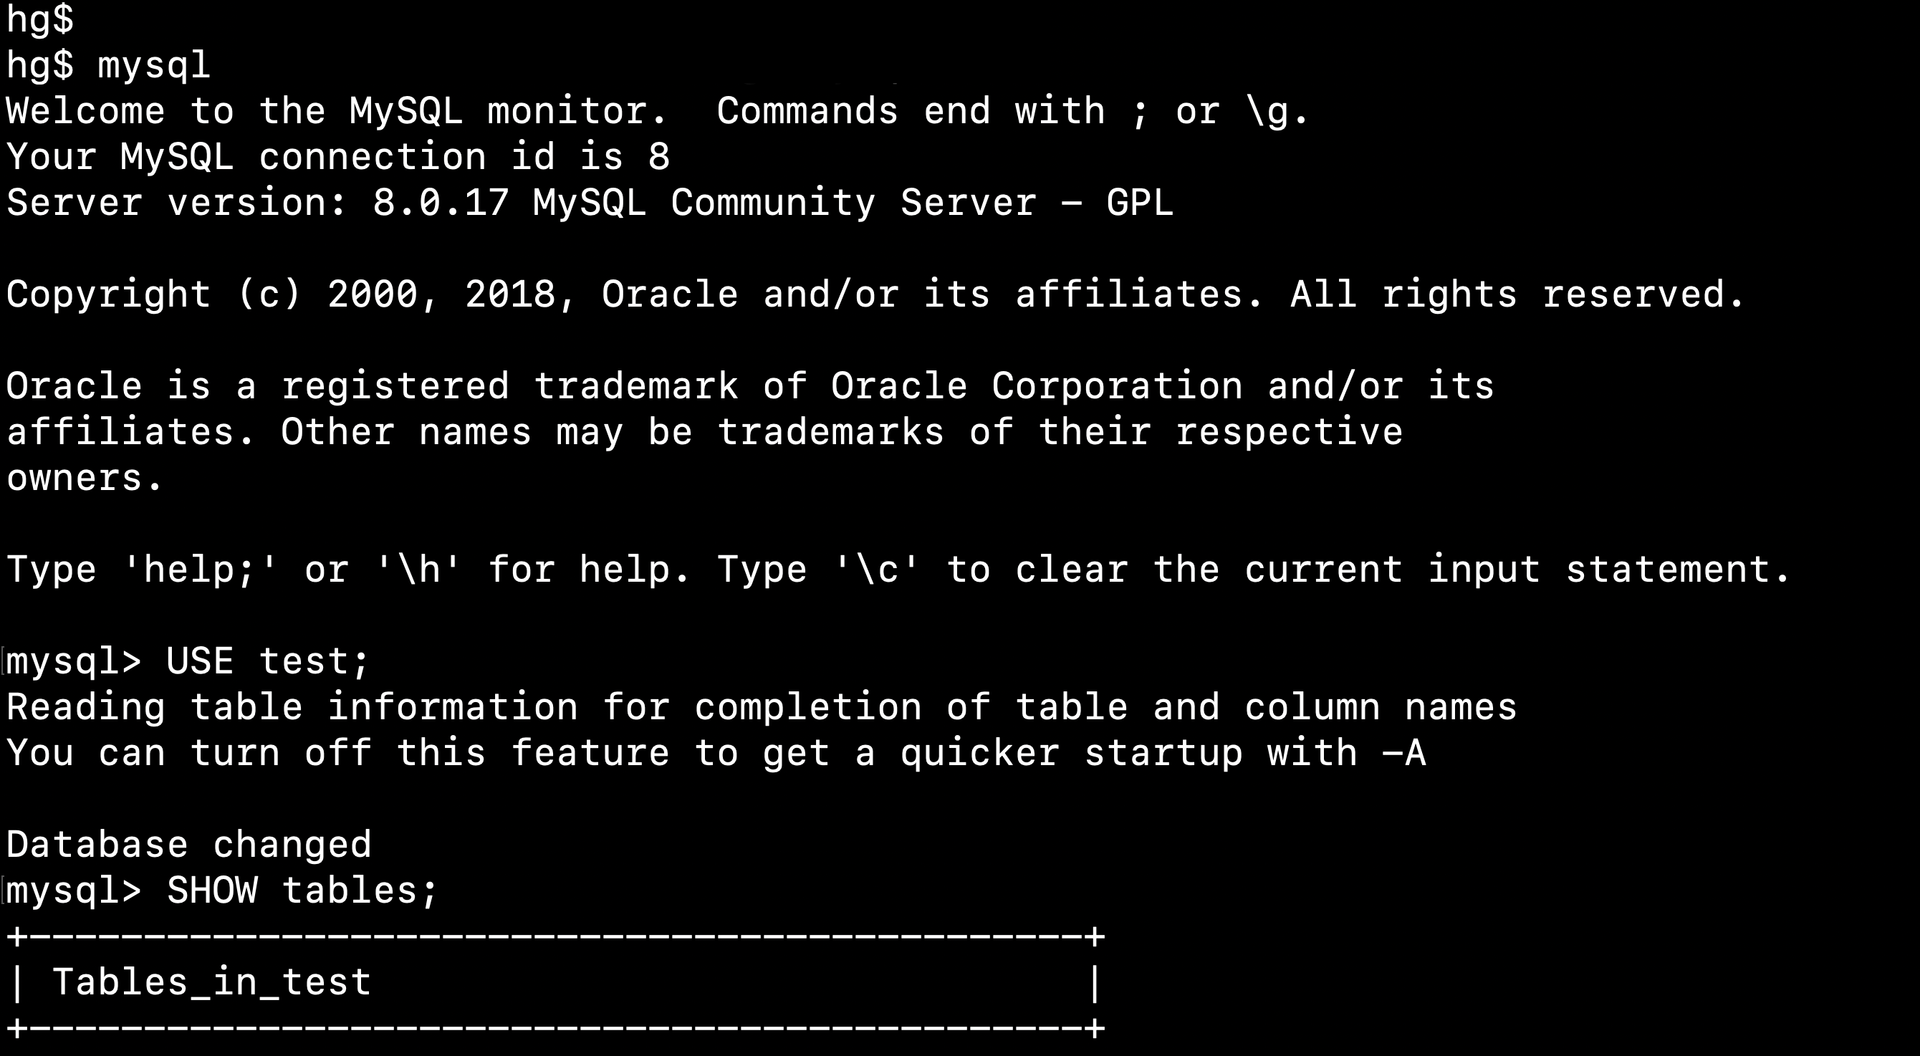
\includegraphics[width=0.8\textwidth]{img/mysqlPres.PNG}
  \caption{Capture d'écran du MySQL par défaut. Source: \href{https://en.wikipedia.org/wiki/MySQL}{Wikipedia}.}
  \label{fig:mysql-image}
\end{figure}

\subsection{Caractéristiques de MySQL}
\begin{itemize}
  \item Open source et gratuit : MySQL est distribué sous la licence GNU General Public License (GPL), ce qui permet aux utilisateurs de l'utiliser, de le modifier et de le distribuer librement.
  \item Haute performance et fiabilité : MySQL est conçu pour être rapide et fiable, avec des fonctionnalités telles que le support des transactions, la réplication, et les sauvegardes en ligne.
  \item Supporte de grandes bases de données : MySQL peut gérer de grandes bases de données avec des millions de lignes et des centaines de tables.
  \item Compatible avec de nombreux systèmes d'exploitation : MySQL fonctionne sur diverses plateformes, y compris Linux, Windows, macOS, et Unix.
  \item Large communauté et support : MySQL bénéficie d'une large communauté d'utilisateurs et de développeurs, ainsi que d'un support commercial fourni par Oracle.
\end{itemize}

\subsection{Architecture de MySQL}
MySQL utilise une architecture client-serveur, où le serveur MySQL gère les bases de données et les clients MySQL se connectent au serveur pour exécuter des requêtes SQL. L'architecture de MySQL comprend plusieurs composants clés :
\begin{itemize}
  \item \textbf{Serveur MySQL} : Le serveur MySQL est le cœur du système, responsable de la gestion des bases de données, de l'exécution des requêtes SQL, et de la gestion des transactions.
  \item \textbf{Connecteurs} : MySQL fournit des connecteurs pour différents langages de programmation, tels que PHP, Python, Java, et C++, permettant aux développeurs de créer des applications qui interagissent avec MySQL.
  \item \textbf{Outils de gestion} : MySQL inclut des outils de gestion tels que MySQL Workbench, un environnement de développement intégré (IDE) pour la conception, le développement et l'administration de bases de données MySQL.
  \item \textbf{Moteurs de stockage} : MySQL supporte plusieurs moteurs de stockage, tels que InnoDB et MyISAM, qui offrent différentes fonctionnalités et performances pour répondre aux besoins spécifiques des applications.
\end{itemize}

\subsection{Utilisations de MySQL}
MySQL est utilisé dans une variété d'applications et de secteurs, notamment :
\begin{itemize}
  \item \textbf{Applications web} : MySQL est souvent utilisé avec des langages de script côté serveur comme PHP pour créer des sites web dynamiques et des applications web.
  \item \textbf{Systèmes de gestion de contenu (CMS)} : De nombreux CMS populaires, tels que WordPress, Joomla, et Drupal, utilisent MySQL comme base de données principale.
  \item \textbf{Applications d'entreprise} : MySQL est utilisé dans des applications d'entreprise pour la gestion des données, les systèmes de gestion de la relation client (CRM), et les systèmes de planification des ressources d'entreprise (ERP).
  \item \textbf{Analytique et Big Data} : MySQL est utilisé pour l'analyse des données et les applications de Big Data, souvent en combinaison avec des outils tels que Hadoop et Spark.
\end{itemize}

\break\section{Relation entre MySQL et PHP}
PHP (Hypertext Preprocessor) est un langage de script côté serveur conçu pour le développement web. MySQL est souvent utilisé avec PHP pour créer des applications web dynamiques. PHP peut interagir avec MySQL pour exécuter des requêtes SQL, récupérer des données et les afficher sur une page web.

\begin{figure}[H]
  \centering
  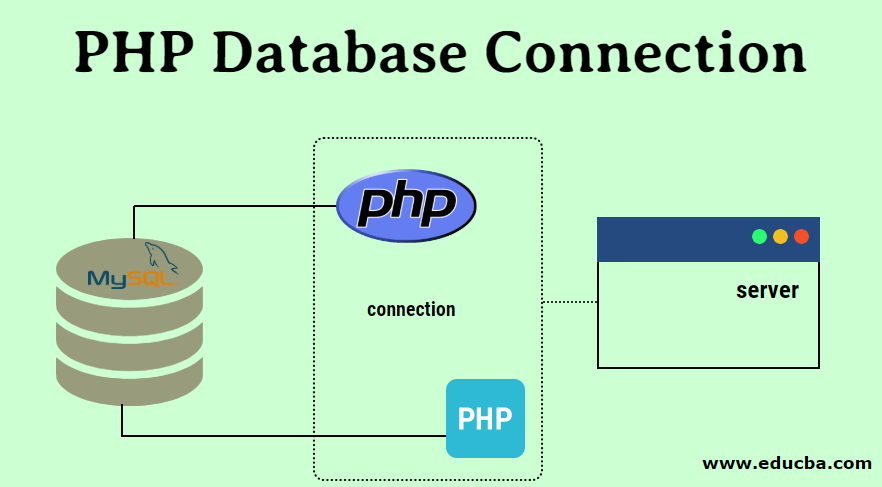
\includegraphics[width=0.8\textwidth]{img/PHP-Database-Connection.png}
  \caption{Connexion entre PHP et MySQL. Source: \href{https://www.educba.com/php-database-connection/}{Educba}.}
  \label{fig:php-mysql-image}
\end{figure}

\subsection{Exemple de connexion PHP à MySQL}
\begin{verbatim}
<?php
$servername = "localhost";
$username = "username";
$password = "password";
$dbname = "database";

// Créer une connexion
$conn = new mysqli($servername, $username, $password, $dbname);

// Vérifier la connexion
if ($conn->connect_error) {
  die("Connection failed: " . $conn->connect_error);
}
echo "Connected successfully";
?>
\end{verbatim}

\section{Conclusion}
SQL est un langage essentiel pour la gestion des bases de données relationnelles, et MySQL est l'un des SGBDR les plus populaires. La combinaison de MySQL et PHP permet de créer des applications web puissantes et dynamiques.

\printbibliography

\end{document}